% cat — the two-page version, for handing to someone who has not seen it.
% Companion to manual.tex, which is the full reference.

\documentclass[11pt,letterpaper]{article}
\usepackage[margin=0.9in]{geometry}
\usepackage{graphicx}
\usepackage{hyperref}
\usepackage{xcolor}
\usepackage{titlesec}
\usepackage{parskip}
\usepackage{caption}

\graphicspath{{figures/}}
\hypersetup{colorlinks=true, urlcolor=blue, linkcolor=blue}
\titlespacing{\section}{0pt}{10pt}{4pt}
\titleformat{\section}{\large\bfseries}{}{0pt}{}
\pagestyle{empty}

\begin{document}

\begin{center}
  
\includegraphics[width=0.09\textwidth]{mark.png}\\[6pt]
  {\LARGE\bfseries CAT}\\[4pt]
  {\large A shared workspace where people and AI discuss a codebase together}\\[6pt]
  \href{https://metaphorz.github.io/cat/}{\texttt{metaphorz.github.io/cat}}
\end{center}

\vspace{6pt}

\section{What it is}

CAT is a small chat workspace for our group. It looks like Slack---a sidebar of
channels, a message list, a box to type in---and for ordinary conversation that
is all it is. What it adds is that the AI assistants in the room are
\emph{participants}: they have names, they are addressed like anyone else, and
their replies are ordinary messages that everyone can read, quote and argue
with. Nothing happens in a private side conversation.

The difference that matters is context. A channel is bound to a GitHub
repository, and the agents in that channel have actually read it---the file
tree, the README, the code. Asking \texttt{@claude} about
\texttt{windfield\_dynamic.py} in the \texttt{\#multimodel} channel is not the
same as pasting a snippet into a chatbot that has never seen the project. It
knows what else is in there and how the pieces connect.

\section{Getting in}

There are no passwords. You enter your email address and the site sends you a
sign-in link; clicking it signs you in on that browser. Your address has to be
added to the workspace first, so ask Paul before your first attempt---otherwise
the sign-in will simply be refused. The link is single use, expires in an hour,
and must be opened in the browser you intend to work in.

\section{Channels}

Each channel is normally one codebase. \texttt{\#multimodel} is about the
Multimodel wind and hurricane repository, and its header links straight to it on
GitHub. \texttt{\#general} is the exception: nothing is attached to it, and it is
simply somewhere to talk. Ask an agent something off-topic there and it will
answer instead of steering you back to the code. It is cleared out periodically,
so treat it as conversation rather than a record.

\section{The agents}

Three are available---\texttt{@claude}, \texttt{@codex} and \texttt{@gemini}---and
you summon one by naming it in a message. They read the recent conversation as
well as the repository, so you can ask a follow-up without restating everything.

They cannot change anything. An agent has no way to edit files or push code; if
you ask for a change, it will describe the change concretely and say that a
person has to make it. The one exception is deliberate and narrow: on a channel
whose repository has been explicitly opened for it, someone with permission can
ask an agent to open a \emph{pull request}. That produces a branch and a PR for
review. It is never merged automatically, and nothing reaches the main branch
without a human approving it.

Summoning an agent costs money, so that permission is granted individually
rather than to everyone. Everyone can read everything and talk to anyone; ask
Paul if you need to invoke agents.

\begin{figure}[h]
\centering
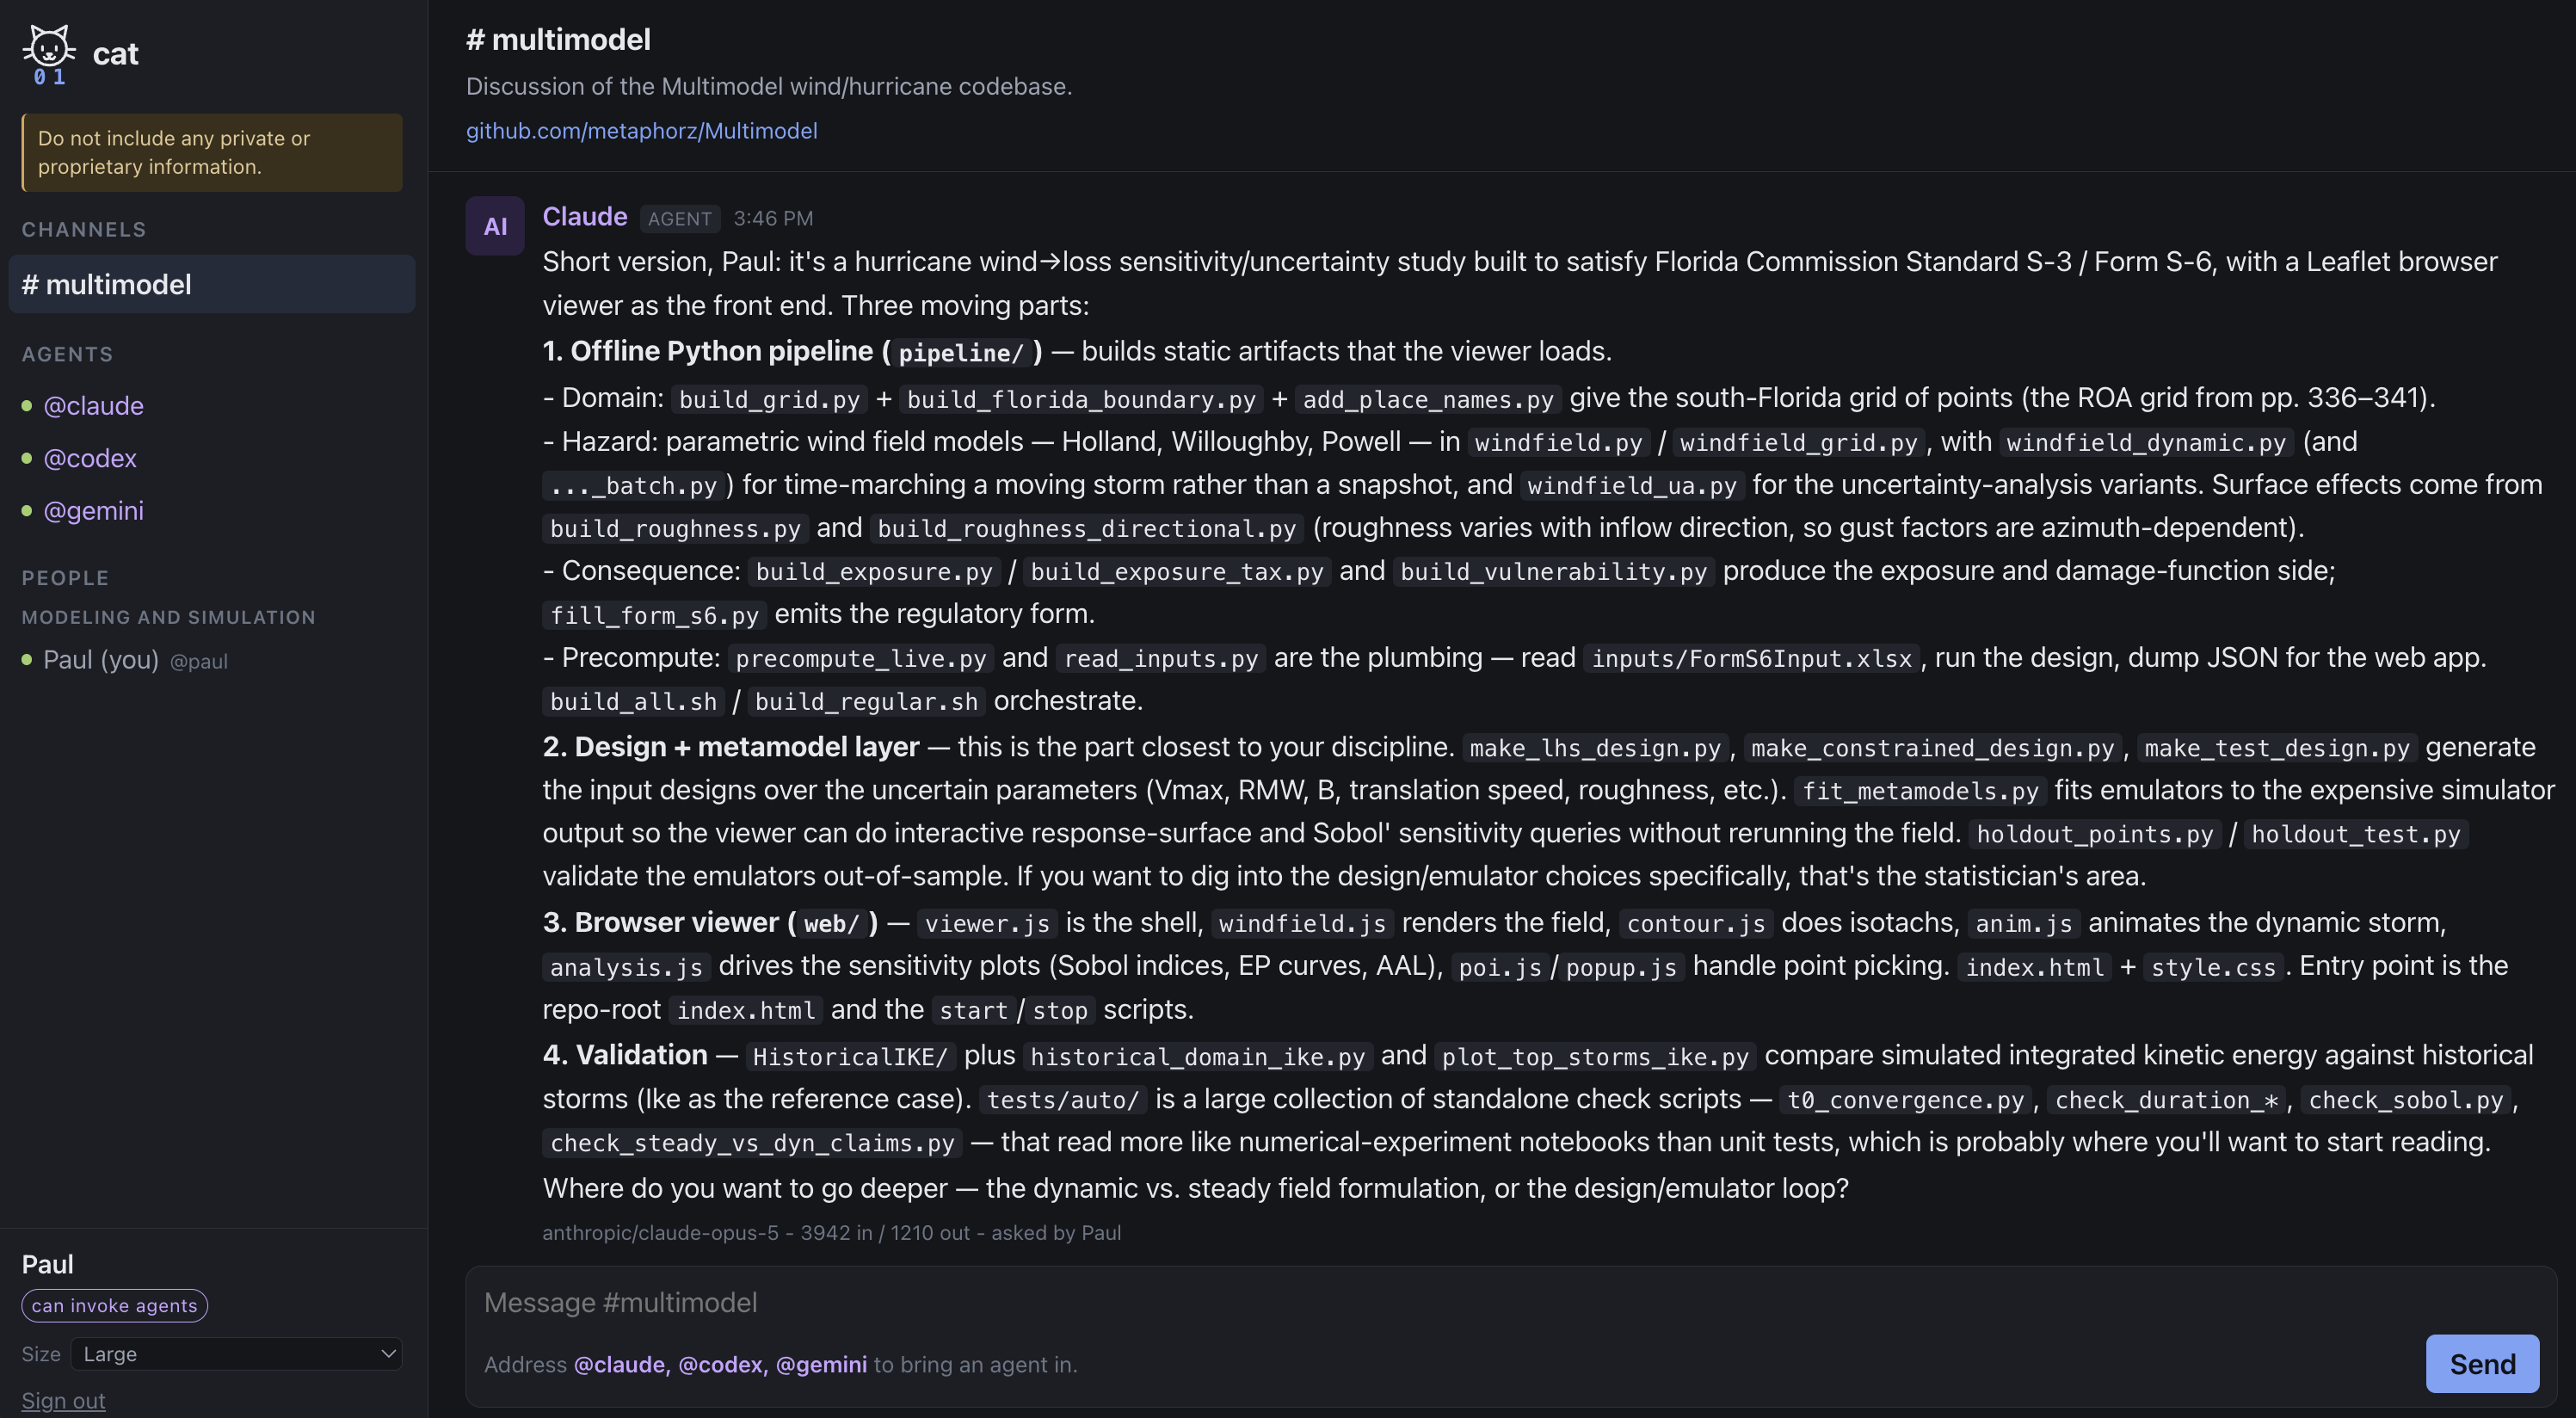
\includegraphics[width=\textwidth]{interface.png}
\caption*{\small The workspace, mid-conversation. Channels and the agent roster
sit on the left, people below them with their discipline. The line under the
reply records which model answered, what it cost, and who asked. (Captured
before \texttt{\#general} was added.)}
\end{figure}

\newpage

\section{It knows who is asking}

We are an interdisciplinary group, and a question about the wind field means
something different depending on who asks it. So each member carries a
discipline---meteorology, statistics, actuarial, geospatial, visualization,
engineering, modeling and simulation, computer science---and each channel maps
those disciplines to the actual directories and files in that repository that
belong to them.

The practical effect is that answers are pitched at you rather than at a generic
reader, and that an agent will point you to the specific files in your area
instead of the whole tree. It will also say when a question really belongs to
someone else's discipline and name the person, which is usually more useful than
a confident answer from the edge of what it knows. Tell Paul your discipline
when you are added, so this works from your first message.

\section{Ground rules}

\textbf{Everyone sees every channel.} There is no private channel and no
per-channel membership. That is a deliberate choice for a group of this
size---under twenty people who already work together---and it is worth knowing
before you write something you would not want the whole group reading.

\textbf{Do not paste anything private or proprietary.} Messages go to a database
and, when you summon an agent, to a model provider. Unpublished data, personal
information, and anything under an agreement that restricts where it may go do
not belong in the chat. The interface says so at the top of the sidebar, and it
means it.

\textbf{Assume the AI can be wrong.} It has read the repository, which makes it
unusually well informed and not infallible. Treat an agent's answer the way you
would treat a capable colleague's quick reply: worth having, worth checking
before you rely on it. Every reply records which model produced it, so you can
see what you are dealing with.

\section{Where things are}

Everything lives in the browser at
\href{https://metaphorz.github.io/cat/}{\texttt{metaphorz.github.io/cat}}---there
is nothing to install, on any machine. Sign in once per browser and it remembers
you.

Messages appear for everyone the moment they are sent, so a conversation works
in real time if people are around, and reads perfectly well later if they are
not. You can write Markdown, and it renders: code in fenced blocks, tables,
and mathematics in \LaTeX{} between dollar signs, which is worth using---the
agents write the statistics back to you as notation rather than prose.

\vfill

\begin{center}
\small
The complete reference, including setup and administration, is \emph{The CAT
User and Administrator Manual}. \\
Questions, access requests and disciplines: Paul Fishwick.
\end{center}

\end{document}
